\chapter{Imunitas Bawaan dan Peradangan}\label{ch:b3:innate-immunity}

Sebuah serpihan di bawah kulit memasukkan sepuluh ribu bakteri yang akan
berganda tiap setengah jam. Dalam hitungan menit pembuluh di sekelilingnya
melebar lalu bocor; dalam sejam \omterm{def:b3:innate-immunity:innate}{neutrofil} yang pertama telah memeras keluar
dari darahnya lalu merangkak ke arah penyusupnya sepanjang sebuah jejak kimia;
dalam sehari tempatnya merah, panas, bengkak, dan nyeri --- keempat
tanda \omterm{def:b3:innate-immunity:inflammation}{peradangan} yang didaftar Celsus dua ribu tahun lalu --- dan
bakterinya mati, dimakan hidup-hidup oleh sel yang mengenalinya sebagai
asing tanpa pernah menjumpainya sebelum itu. Inilah \omterm{def:b3:innate-immunity:innate}{imunitas bawaan}:
pertahanan yang dipunyai tiap hewan, siap sebelum infeksinya, yang disandi di
dalam genom alih-alih dipelajari. Ia cepat, ia yang membunuh kebanyakan
penyerbu, dan ia yang memberi tahu imunitas terpelajar bab berikutnya yang
lebih lambat bahwa ada sesuatu yang harus dipelajari. Keberlebihannya ---
renjatan septik, \omterm{def:b3:innate-immunity:inflammation}{peradangan} menahun, demam penyakit autoradang --- sama
mengajarkan seperti keberhasilannya.

\section{Lapisan dan sel}

\begin{definition}[Imunitas bawaan]\label{def:b3:innate-immunity:innate}
\index{imunitas bawaan}\index{neutrofil}\index{makrofag}%
\index{sel dendritik}\index{sel pembunuh alami}\index{penghadang}
\emph{Imunitas bawaan} adalah himpunan pertahanan yang hadir sebelum
pemaparan apa pun, yang disandi gen nutfah yang tidak menyusun ulang diri, yang
mengenali ciri lestari mikroba alih-alih perseorangan tertentu, yang bekerja
dalam hitungan menit sampai jam, dan (dengan syarat) tanpa ingatan. Lapisan
pertamanya adalah \emph{penghadang}: keratin kulit, lendir dan
\omterm{def:b3:cytoskeleton-motility:cilia}{silium} saluran napas, asam lambung, pembilasan kemih
dan air mata, enzim lisozim yang memotong \omterm{def:b3:bacteriology:envelope}{peptidoglikan},
\emph{peptida antimikroba} (defensin, katelisidin) yang melubangi
selaput mikroba, serta \omterm{def:b3:microbiomes:symbiosis}{mikrobiom} komensal yang menempati
ceruknya (\cref{ch:b3:microbiomes}). Selnya, semuanya dari garis
keturunan mieloid kecuali yang terakhir: \emph{neutrofil}, yakni \qty{60}{\%}
leukosit darah, $10^{11}$ dibuat sehari, hidup sehari, yang pertama tiba dan
pembunuh utama bakteri; \emph{makrofag}, penghuni tiap jaringan yang
berumur panjang (sel Kupffer di hati, mikroglia di otak,
makrofag alveolus di paru) yang makan, membersihkan, dan membunyikan
lonceng bahaya; \emph{sel dendritik}, yang mencontoh jaringan lalu mengusung
temuannya ke kelenjar limfa; sel mast, basofil, dan eosinofil, yang bersenjata
melawan parasit dan bertanggung jawab atas alergi; serta \emph{sel pembunuh
alami} (NK), yakni limfosit yang membunuh sel terinfeksi atau terubah begitu
melihatnya.
\end{definition}

\begin{proof}[Bukti eksperimental]
Metchnikoff (1882), di Messina, menusukkan sebuah duri mawar ke dalam sebuah
larva bintang laut yang bening lalu menyaksikan, keesokan paginya, sel yang
bergerak berkerumun di sekelilingnya; ia telah melihat sel yang sama menelan
butir makanan dan butir zat warna, lalu mengusulkan bahwa sel itu menelan
mikroba juga --- itulah \emph{fagosit}, pelaku sebuah pertahanan inang yang
kemudian ia telusuri pada tiap hewan yang dapat ia temukan, dari amoeba sampai
manusia. Ia berbagi hadiah Nobel tahun 1908 dengan Ehrlich, yang antibodinya
mewakili pandangan humoral yang berlawanan; keduanya benar, dan seabad kemudian
kedua paruh imunitas itu terbukti satu sistem, dengan paruh bawaan mengajari
yang adaptif.
\end{proof}

\begin{omfigure}
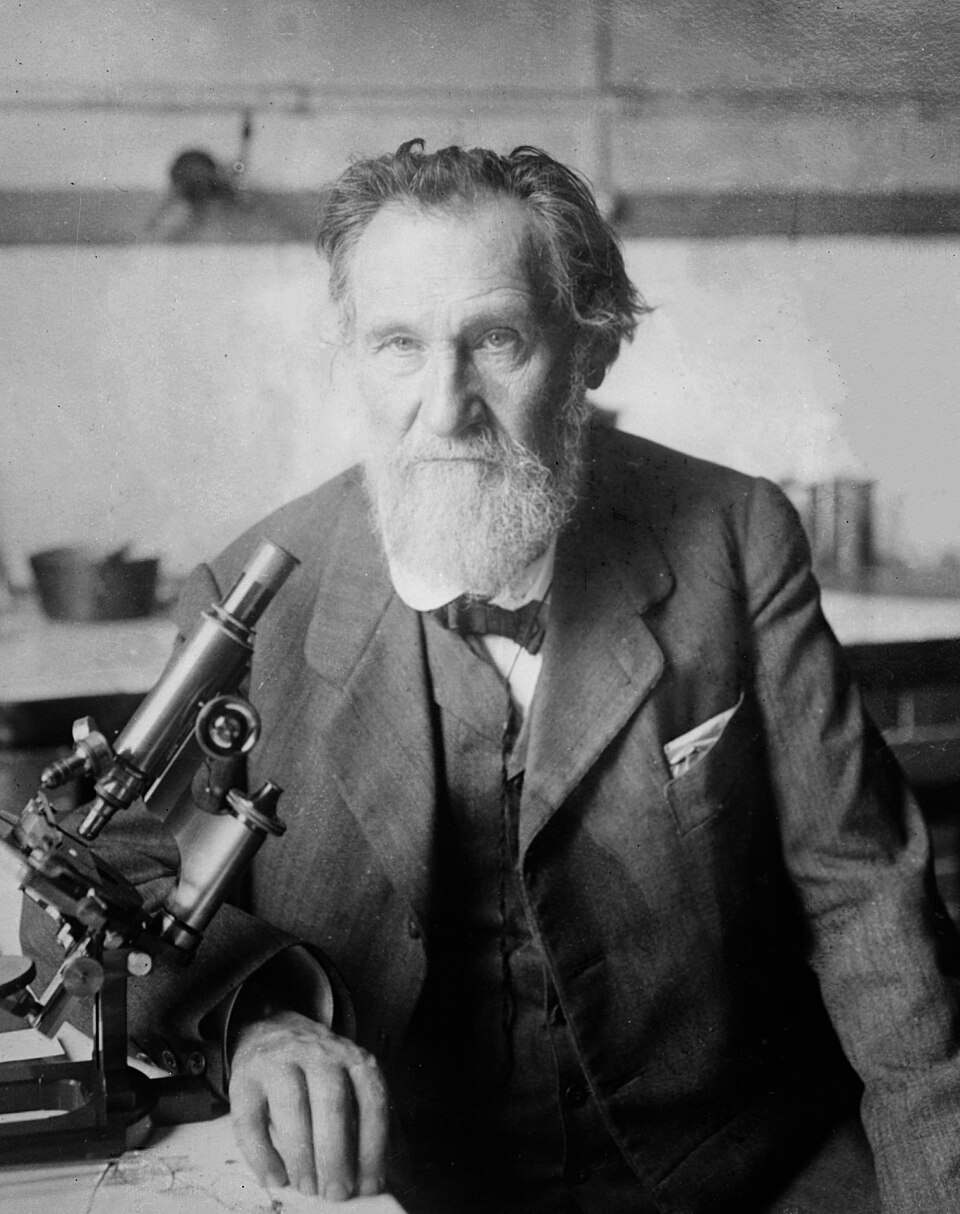
\includegraphics[width=0.30\linewidth]{images/book5/metchnikoff.jpg}\hspace{0.04\linewidth}
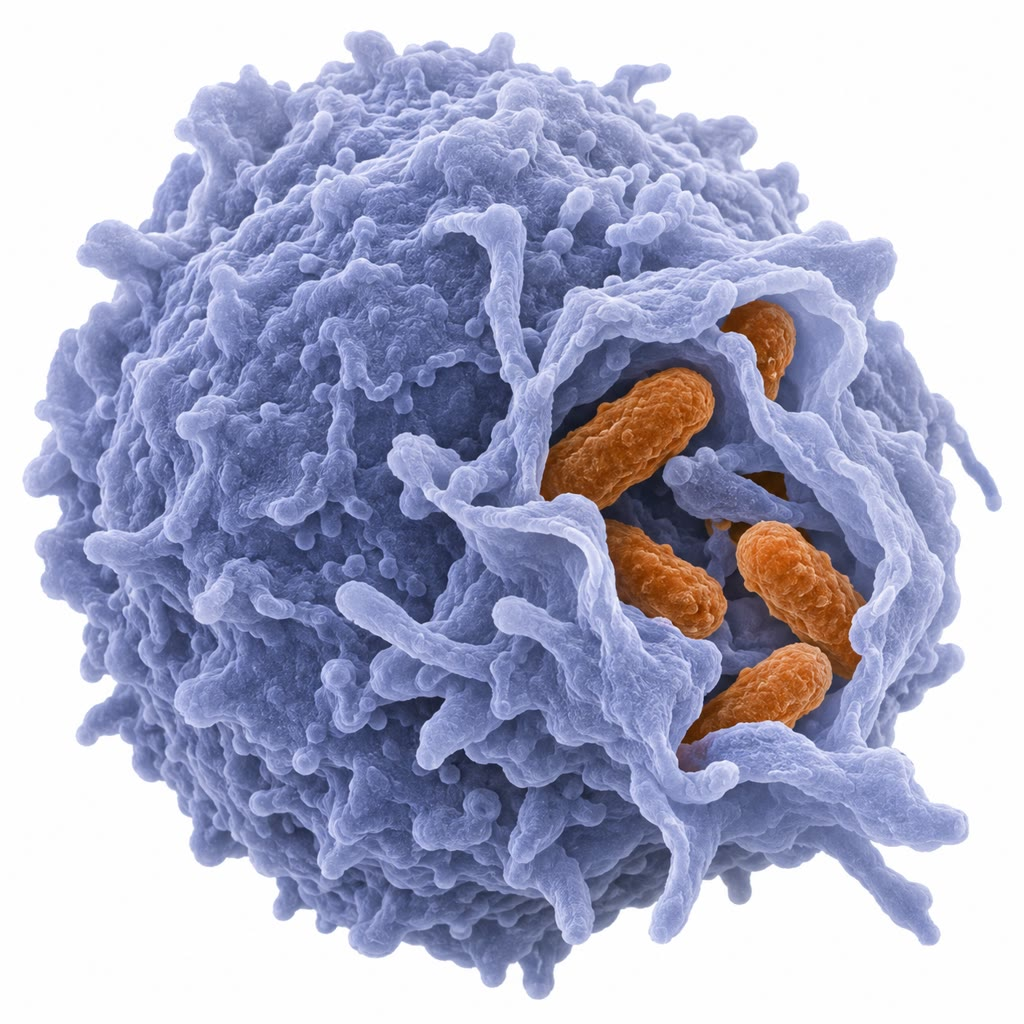
\includegraphics[width=0.30\linewidth]{images/book5/ai/b5-15-neutrophil-phagocytosis.jpg}\hspace{0.04\linewidth}
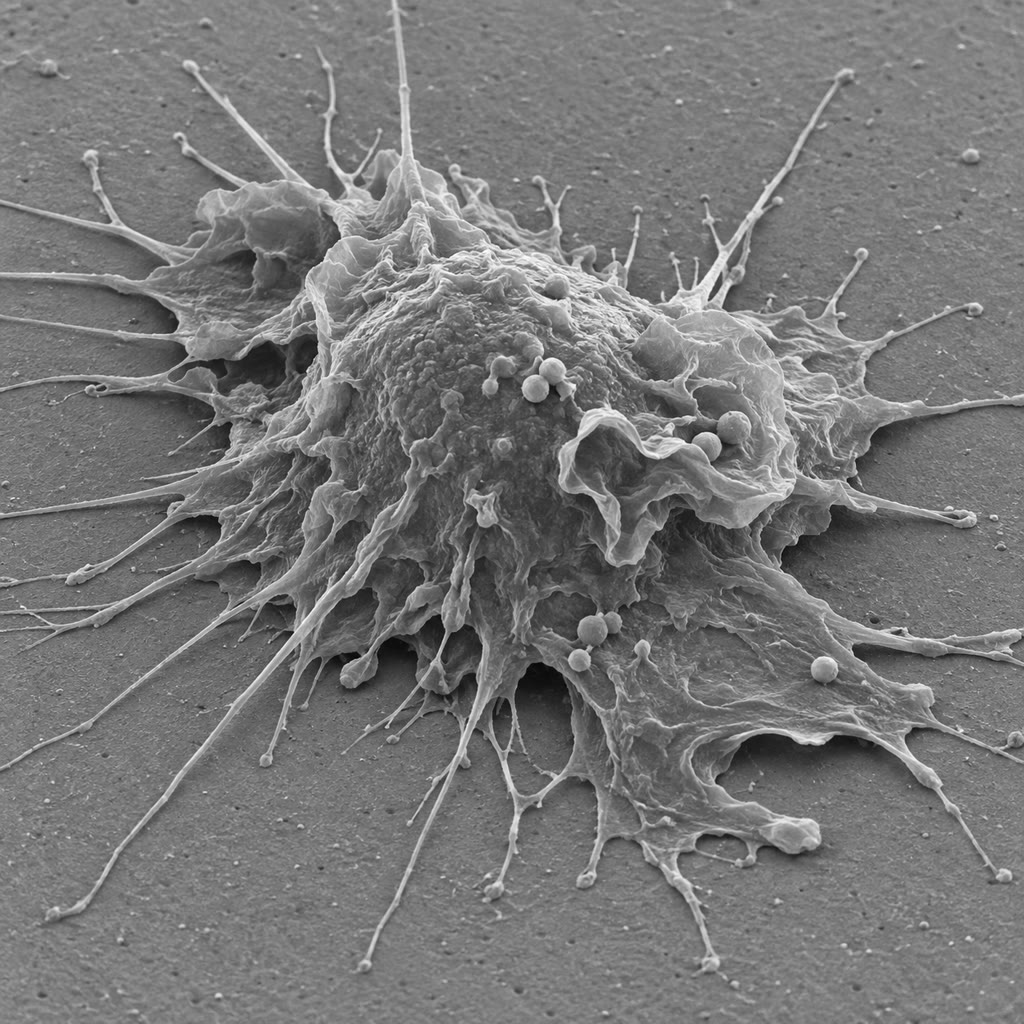
\includegraphics[width=0.30\linewidth]{images/book5/ai/b5-15-macrophage.jpg}

{\small Élie Metchnikoff, yang menyaksikan fagosit berkumpul di sekeliling
sebuah duri di dalam larva bintang laut lalu mendirikan imunologi sel
(Perpustakaan Kongres, domain publik). Tengah: sebuah \omterm{def:b3:innate-immunity:innate}{neutrofil} menelan bakteri.
Kanan: sebuah \omterm{def:b3:innate-immunity:innate}{makrofag} menebarkan selaput berkerutnya di atas sebuah permukaan.}
\end{omfigure}

\section{Mengenali musuh}

\begin{definition}[Pengenalan pola]\label{def:b3:innate-immunity:prr}
\index{reseptor pengenal pola}\index{pola molekul terkait patogen}%
\index{reseptor serupa Toll}%
\index{pola molekul terkait kerusakan}\index{inflamasom}
Sel bawaan mengenali \emph{pola molekul terkait patogen}
(PAMP): molekul yang lazim pada seluruh kelas mikroba, yang penting bagi
mereka, dan yang tidak ada pada inangnya --- \omterm{def:b3:bacteriology:envelope}{lipopolisakarida} dinding
\omterm{def:b3:bacteriology:envelope}{Gram-negatif}, \omterm{def:b3:bacteriology:envelope}{peptidoglikan} dan asam lipoteikoat pada \omterm{def:b3:bacteriology:envelope}{Gram-positif},
flagelin, $\beta$-glukan jamur, RNA untai ganda, RNA tanpa
tudung 5$'$, DNA dengan \omterm{def:b3:chromatin-epigenetics:methylation}{CpG} tak termetilasi, DNA di dalam sitosol. Reseptornya
adalah \emph{reseptor pengenal pola} (PRR), beberapa lusin saja seluruhnya,
masing-masing disandi satu gen: \emph{reseptor serupa Toll} (TLR) pada
permukaan dan di dalam \omterm{def:b3:membrane-traffic:endocytosis}{endosom} (TLR4 bagi \omterm{def:b3:bacteriology:envelope}{lipopolisakarida}, TLR5 bagi
flagelin, TLR3 bagi RNA untai ganda, TLR9 bagi DNA \omterm{def:b3:chromatin-epigenetics:methylation}{CpG}); protein
NOD sitosolik bagi serpihan \omterm{def:b3:bacteriology:envelope}{peptidoglikan}, RIG-I bagi RNA
\omterm{def:b3:virology:virus}{virus}, cGAS--STING bagi DNA sitosolik; lektin jenis C bagi gula jamur.
Reseptor yang sama, atau reseptor lain dari keluarga yang sama, mengenali
\emph{pola molekul terkait kerusakan} (DAMP) yang dilepaskan oleh sel
yang terluka --- ATP, asam urat, protein inti HMGB1, dan DNA
mitokondria --- sehingga cedera steril pun meradang. Pengikatannya mengaktifkan
faktor transkripsi NF-$\kappa$B dan faktor pengatur interferon,
yang menyalakan \omterm{def:b3:innate-immunity:inflammation}{sitokin}, \omterm{def:b3:innate-immunity:inflammation}{kemokin}, molekul pelekat, dan
gen antimikroba dalam sejam; sebagian pengindera sitosolik
merakit \emph{inflamasom}, yakni sebuah landasan yang mengaktifkan kaspase-1
untuk memotong interleukin-1$\beta$ menjadi bentuk aktifnya lalu memicu
kematian meradang yang disebut \omterm{def:b3:cell-cycle-apoptosis:other}{piroptosis} (\cref{ch:b3:cell-cycle-apoptosis}).
\end{definition}

\begin{proof}[Bukti eksperimental]
Janeway mengusulkan pada tahun 1989 bahwa sistem imun adaptif tidak
menanggapi antigen saja melainkan memerlukan sebuah isyarat dari reseptor bawaan
yang telah mengenali pola mikroba --- itulah penjelasan mengapa vaksin
memerlukan ajuvan, ``rahasia kotor kecil sang imunolog''. Hoffmann
(1996) menemukan bahwa \emph{Drosophila} yang tidak punya reseptor Toll, yang
dikenal karena perannya pada pemolaan embrio, tidak dapat menegakkan sebuah
tanggapan antijamur lalu mati bersalut kapang; Beutler (1998) memetakan
ketahanan sebuah galur mencit terhadap \omterm{def:b3:bacteriology:envelope}{lipopolisakarida}, yang selamat dari dosis
endotoksin yang mematikan bagi yang lain namun gagal membersihkan infeksi
\omterm{def:b3:bacteriology:envelope}{Gram-negatif}, ke sebuah mutasi pada homolog mamalianya TLR4. Reseptor
bagi endotoksin, yang dicari selama lima puluh tahun, ternyata sebuah Toll.
\end{proof}

\begin{omfigure}
\begin{tikzpicture}[every node/.style={font=\scriptsize}, >=stealth]
  % membrane
  \draw[very thick, omDef] (0,3.0) -- (11.5,3.0); \draw[very thick, omDef] (0,2.7) -- (11.5,2.7);
  \node[above] at (0.5,3.05) {luar}; \node[below] at (0.5,2.65) {sitosol};
  % TLR4 with LPS
  \draw[thick, fill=omProp!35] (2.2,2.4) rectangle (2.6,3.9); \draw[thick, fill=omProp!35] (2.9,2.4) rectangle (3.3,3.9);
  \fill[omThm] (2.75,4.1) circle (0.14); \node[above] at (2.75,4.25) {LPS (sebuah PAMP)};
  \node[right, align=left] at (3.4,3.5) {dimer TLR4\\dengan MD2};
  % signalling
  \node[draw, thick, rounded corners, fill=omDef!20] (myd) at (2.75,1.7) {MyD88, kinase};
  \node[draw, thick, rounded corners, fill=omDef!20] (nfkb) at (2.75,0.6) {NF-$\kappa$B terlepas};
  \node[draw, thick, rounded corners, fill=omMeth!25, align=center] (genes) at (2.75,-0.8) {TNF, IL-1$\beta$, IL-6, IL-8;\\molekul pelekat; iNOS};
  \draw[->, thick] (2.75,2.4) -- (myd); \draw[->, thick] (myd) -- (nfkb); \draw[->, thick] (nfkb) -- (genes);
  \node[right, font=\tiny] at (3.3,1.2) {dalam sejam};
  % cytosolic sensors
  \node[draw, thick, rounded corners, fill=omProp!25, align=center] (rig) at (6.9,1.9) {RIG-I: RNA virus\\cGAS--STING: DNA sitosolik};
  \node[draw, thick, rounded corners, fill=omMeth!25] (ifn) at (6.9,-0.2) {interferon jenis I};
  \draw[->, thick] (rig) -- node[midway, right] {IRF3, IRF7} (ifn);
  \node[draw, thick, rounded corners, fill=omThm!20, align=center] (nlrp) at (10.9,1.9) {inflamasom NLRP3:\\hablur, ATP, liang};
  \node[draw, thick, rounded corners, fill=omMeth!25, align=center] (il1) at (10.9,-0.8) {kaspase-1: IL-1$\beta$\\terlepas; piroptosis};
  \draw[->, thick] (nlrp) -- (il1);
  \draw[->, thick, dashed] (genes.south) -- ++(0,-0.5) -| (il1.south) node[pos=0.25, below, font=\tiny] {pro-IL-1$\beta$ dipasok jalur TLR};
\end{tikzpicture}

{\small Tiga lengan pengenalan pola. Sebuah \omterm{def:b3:innate-immunity:prr}{reseptor serupa Toll} di
permukaan yang diikat \omterm{def:b3:bacteriology:envelope}{lipopolisakarida} berisyarat lewat NF-$\kappa$B ke
\omterm{def:b3:innate-immunity:inflammation}{sitokin} \omterm{def:b3:innate-immunity:inflammation}{peradangan}; pengindera sitosolik asam nukleat \omterm{def:b3:virology:virus}{virus} memicu
interferon; \omterm{def:b3:innate-immunity:prr}{inflamasomnya} mengubah pendahulu tersimpan
interleukin-1 menjadi \omterm{def:b3:innate-immunity:inflammation}{sitokin} yang aktif.}
\end{omfigure}

\begin{definition}[Komplemen]\label{def:b3:innate-immunity:complement}
\index{komplemen}\index{konvertase C3}\index{opsonisasi}%
\index{kompleks penyerang membran}\index{anafilatoksin}
\emph{Komplemen} adalah sebuah sistem berisi sekitar tiga puluh protein plasma,
yakni \qty{10}{\%} globulin serum, yang menandai lalu memusnahkan mikroba
dengan sebuah runtunan pengaktifan proteolitik. Tiga jalur bertemu pada
pemotongan protein pusatnya C3: jalur \emph{klasik},
yang dimulai C1q yang mengikat antibodi pada sebuah permukaan (atau \omterm{prop:b3:innate-immunity:systemic}{protein
C-reaktif}, atau sel yang berapoptosis); jalur \emph{lektin}, yang dimulai
lektin pengikat manosa yang mengenali gula mikroba; dan
jalur \emph{alternatif}, yang di dalamnya C3 terhidrolisis dengan sendirinya pada
laju rendah lalu C3b yang dihasilkannya melekat pada permukaan apa pun yang
dijumpainya. Tiap jalur membangun sebuah \emph{konvertase C3}, yakni enzim yang
memotong lebih banyak C3; C3b yang diendapkannya secara kovalen pada permukaan
itu membangun lebih banyak konvertase pada gilirannya --- sebuah gelung
pelipatgandaan --- sehingga sebuah bakteri tersalut jutaan C3b dalam hitungan
menit. C3b adalah sebuah \emph{opsonin}: fagosit mengusung reseptor baginya lalu
memakan apa pun yang disalutinya. Serpihan kecilnya C3a dan C5a adalah
\emph{anafilatoksin} yang melebarkan pembuluh, menarik
\omterm{def:b3:innate-immunity:innate}{neutrofil}, dan mengaktifkan sel mast. Lalu C5b merakit C6--C9 menjadi
\emph{kompleks penyerang membran}, yakni sebuah liang \qty{10}{nm} yang
melisiskan bakteri \omterm{def:b3:bacteriology:envelope}{Gram-negatif} dan \omterm{def:b3:virology:virus}{virus} berselubung. Sel inang terluput
karena ia mengusung pengatur --- faktor H, CD55, CD59 --- yang
membongkar konvertasenya lalu menghalangi liangnya pada permukaannya sendiri;
mikroba, yang tidak punya itu, dimakan habis oleh gelungnya.
\end{definition}

\begin{theorem}[Gelung komplemen sebagai pembeda kinetik]\label{thm:b3:innate-immunity:complement}
\index{komplemen!gelung pelipatgandaan}
Misalkanlah $B(t)$ cacah molekul C3b yang diendapkan pada sebuah permukaan. C3b
diendapkan pada laju tetap yang kecil $k_{0}$ dari denyut sendiri
C3, dan tiap C3b yang mengendap membangun konvertase yang mengendapkan lebih
banyak pada laju $a$ tiap C3b tiap detik, sementara pengatur (inang) dan
peluruhan menyingkirkan keaktifan konvertase pada laju $d$ tiap C3b tiap detik:
\[
\frac{\mathrm{d}B}{\mathrm{d}t} = k_{0} + (a - d)\,B .
\]
Pada sebuah permukaan yang $a > d$ --- yakni sebuah mikroba, tanpa pengatur ---
$B(t) = \bigl[k_{0}/(a-d)\bigr]\bigl(e^{(a-d)t} - 1\bigr)$ tumbuh
secara eksponensial dengan tetapan waktu $1/(a - d)$; pada permukaan inang yang
$d > a$, $B$ mendekati nilai mantap yang kecil $k_{0}/(d - a)$. Molekul
yang sama, pada kepekatan yang sama, mengendapkan sejuta C3b pada sebuah
bakteri dalam beberapa menit dan beberapa lusin pada sel di sebelahnya:
pembedaan antara diri dan bukan-diri dibuat bukan oleh pengenalan melainkan oleh
tanda $a - d$.
\end{theorem}
\begin{proof}
Persamaannya linear dengan koefisien tetap. Bagi $a \ne d$ titik
tetapnya adalah $B^{*} = -k_{0}/(a-d)$; dengan menulis $B = B^{*} + u$,
$\mathrm{d}u/\mathrm{d}t = (a-d)u$, sehingga $u = u_{0}e^{(a-d)t}$ dan dengan
$B(0) = 0$, $B(t) = \bigl[k_{0}/(a-d)\bigr](e^{(a-d)t} - 1)$. Bagi $a > d$
ini tumbuh tanpa batas (sampai C3 atau permukaannya habis); bagi $a < d$
eksponensialnya meluruh dan $B \to k_{0}/(d-a) > 0$. Dengan $k_{0} = 1$
tiap detik, $a - d = \qty{0.1}{s^{-1}}$ pada sebuah bakteri, $B(\qty{2}{min})
= 10(e^{12} - 1) \approx 1.6\times 10^{6}$; dengan $d - a =
\qty{0.1}{s^{-1}}$ pada sebuah sel inang, $B^{*} = 10$.
\end{proof}

\begin{omfigure}
\begin{tikzpicture}
\begin{axis}[
  width=0.66\linewidth, height=5.6cm,
  axis x line=bottom, axis y line=left,
  xmin=0, xmax=150, ymin=1, ymax=1e7, ymode=log,
  xlabel={detik}, ylabel={C3b yang mengendap},
  xlabel style={font=\small, at={(axis description cs:0.5,-0.12)}, anchor=north}, ylabel style={font=\small},
  tick label style={font=\small}, xtick={0,30,60,90,120,150},
  clip=false,
]
\addplot[very thick, omThm, domain=1:150, samples=80] {10*(exp(0.1*x)-1)};
\addplot[very thick, omDef, domain=1:150, samples=80] {10*(1-exp(-0.1*x))};
\node[font=\scriptsize, omThm, anchor=east] at (axis cs:100,2e5) {mikroba: $a > d$, eksponensial};
\node[font=\scriptsize, omDef, anchor=south west] at (axis cs:60,14) {sel inang: $d > a$, jenuh pada $k_{0}/(d-a)$};
\end{axis}
\end{tikzpicture}

{\small Gelung \omterm{def:b3:innate-immunity:complement}{komplemen} pada dua permukaan dengan $k_{0} = 1$ tiap detik
dan $|a - d| = \qty{0.1}{s^{-1}}$: pada sebuah mikroba tanpa pengatur, C3b
tumbuh secara eksponensial lalu mencapai sejuta dalam dua menit; pada sebuah sel
inang yang berpengatur, ia mendatar pada sepuluh.}
\end{omfigure}

\begin{omfigure}
\begin{tikzpicture}[every node/.style={font=\scriptsize}, >=stealth]
  \node[draw, thick, rounded corners, fill=omDef!20, align=center] (cl) at (-4.2,3.0) {klasik:\\C1q pada antibodi\\atau protein C-reaktif};
  \node[draw, thick, rounded corners, fill=omDef!20, align=center] (le) at (0,3.0) {lektin:\\lektin pengikat manosa\\pada gula mikroba};
  \node[draw, thick, rounded corners, fill=omDef!20, align=center] (al) at (4.2,3.0) {alternatif:\\denyut sendiri C3,\\C3b pada permukaan apa pun};
  \node[draw, thick, rounded corners, fill=omProp!35, minimum width=3cm] (conv) at (0,1.2) {konvertase C3};
  \node[draw, thick, rounded corners, fill=omThm!25, align=center] (c3b) at (0,-0.4) {C3 $\to$ C3b (pada permukaannya) $+$ C3a};
  \draw[->, thick] (cl) -- (conv); \draw[->, thick] (le) -- (conv); \draw[->, thick] (al) -- (conv);
  \draw[->, thick] (conv) -- (c3b);
  \draw[->, very thick, omThm] (c3b.east) .. controls (3.2,-0.4) and (3.2,1.2) .. (conv.east) node[pos=0.5, right, align=left] {gelung pelipatgandaan:\\C3b membangun lebih banyak konvertase};
  \node[draw, thick, rounded corners, fill=omMeth!25, align=center] (ops) at (-4.4,-2.2) {opsonisasi:\\fagosit memakan\\apa yang disaluti C3b};
  \node[draw, thick, rounded corners, fill=omMeth!25, align=center] (ana) at (0,-2.2) {C3a, C5a:\\pembuluh melebar, neutrofil\\dan sel mast direkrut};
  \node[draw, thick, rounded corners, fill=omMeth!25, align=center] (mac) at (4.4,-2.2) {C5b--C9:\\kompleks penyerang membran,\\lisis};
  \draw[->, thick] (c3b) -- (ops); \draw[->, thick] (c3b) -- (ana); \draw[->, thick] (c3b) -- (mac);
  \node[draw, thick, rounded corners, fill=gray!15, align=center] (reg) at (-4.4,1.2) {pengatur inang:\\faktor H, CD55, CD59};
  \draw[-|, thick, gray!60!black] (reg) -- (conv);
\end{tikzpicture}

{\small \omterm{def:b3:innate-immunity:complement}{Komplemen}. Tiga jalan membangun sebuah \omterm{def:b3:innate-immunity:complement}{konvertase C3}; C3b yang
diendapkannya membangun lebih banyak (gelung teoremanya), lalu C3b yang
mengendap itu mengopsonisasi, serpihannya meradangkan, dan kompleks terminalnya
melisiskan. Sel inang mengusung pengatur yang memotong gelungnya (dan, dengan
CD59, menghalangi liangnya) pada selaputnya sendiri.}
\end{omfigure}

\section{Peradangan}

\begin{definition}[Peradangan akut]\label{def:b3:innate-immunity:inflammation}
\index{peradangan}\index{sitokin}\index{kemokin}%
\index{ekstravasasi}\index{selektin}\index{integrin}
\emph{Peradangan} adalah tanggapan jaringan berpembuluh terhadap cedera atau
infeksi, yang ditata \emph{sitokin} --- yakni protein pengisyarat kecil
milik sel imun, di sini terutama TNF, interleukin-1, dan
interleukin-6 dari \omterm{def:b3:innate-immunity:innate}{makrofag} yang aktif --- dan oleh \emph{kemokin},
yakni sitokin yang mengarahkan perpindahan. Tahapnya menjelaskan tanda Celsus.
Histamin dari sel mast, nitrat oksida, dan prostaglandin melebarkan
arteriol: itulah \emph{kemerahan} dan \emph{panas}. Endotelium
venula mengerut lalu membocorkan plasma, yang proteinnya --- \omterm{def:b3:innate-immunity:complement}{komplemen},
antibodi, faktor pembekuan --- membanjiri jaringannya: itulah \emph{pembengkakan}.
Bradikinin dan prostaglandin E$_{2}$ menajamkan ujung saraf:
itulah \emph{nyeri}. Lalu leukositnya tiba lewat \emph{ekstravasasi}: TNF dan
interleukin-1 membuat endoteliumnya memajang \emph{selektin}, yang padanya
\omterm{def:b3:innate-immunity:innate}{neutrofil} yang lewat tersangkut lalu berguling; kemokin (interleukin-8) pada
permukaan endotelium mengaktifkan \emph{integrin} \omterm{def:b3:innate-immunity:innate}{neutrofilnya}, yang
mengikat erat molekul pelekat endotelium lalu menghentikan selnya; dan
\omterm{def:b3:innate-immunity:innate}{neutrofilnya} memeras di antara sel endotelium lalu mengikuti
landaian kemokin ke dalam jaringannya --- seluruh urutan itu dalam beberapa
menit, pada sampai sejuta sel sejam ke dalam sebuah tempat yang terinfeksi.
\end{definition}

\begin{omfigure}
\begin{tikzpicture}[every node/.style={font=\scriptsize}, >=stealth]
  % vessel wall
  \fill[omThm!10] (0,0) rectangle (12,2.3); \node[left, omThm!70!black, anchor=north east] at (12,2.25) {darah, mengalir $\rightarrow$};
  \foreach \x in {0,1.5,3,4.5,6,7.5,9,10.5} \draw[thick, fill=omDef!30] (\x,-0.05) rectangle (\x+1.45,0.35);
  \node[right] at (0.1,-0.35) {endotelium};
  \fill[omMeth!8] (0,-1.7) rectangle (12,-0.45); \node[right, omMeth!60!black] at (0.1,-1.55) {jaringan};
  % bacteria and chemokine gradient
  \foreach \p in {(10.6,-1.1),(11.0,-0.9),(11.3,-1.2)} \fill[omProp] \p ellipse (0.14 and 0.07);
  \node[below, omProp] at (11.0,-1.35) {bakteri};
  \node[below, font=\tiny] at (8.0,-0.5) {landaian kemokin $\rightarrow$};
  % neutrophils in sequence
  \draw[thick, fill=white] (1.2,1.1) circle (0.3); \node[above] at (1.2,1.45) {1. mengalir};
  \draw[thick, fill=white] (3.4,0.68) circle (0.3); \node[above] at (3.4,1.05) {2. berguling pada selektin};
  \draw[omThm, thick] (3.1,0.45) -- (3.05,0.35); \draw[omThm, thick] (3.4,0.38) -- (3.4,0.35); \draw[omThm, thick] (3.7,0.45) -- (3.75,0.35);
  \draw[thick, fill=white] (6.0,0.62) ellipse (0.38 and 0.26); \node[above, align=center] at (6.0,0.95) {3. pelekatan teguh\\(integrin)};
  \draw[thick, fill=white] (8.25,0.18) ellipse (0.2 and 0.42); \node[above, align=center] at (8.4,0.95) {4. memeras\\menembus};
  \draw[thick, fill=white] (9.6,-1.0) circle (0.3); \node[left] at (9.25,-1.0) {5. merangkak ke tempatnya};
  \draw[->, thick, gray] (1.5,1.05) -- (3.0,0.8); \draw[->, thick, gray] (3.7,0.68) -- (5.6,0.62); \draw[->, thick, gray] (6.4,0.5) -- (8.0,0.4); \draw[->, thick, gray] (8.3,-0.3) -- (9.3,-0.8);
  % TNF label
  \node[below, align=center, font=\tiny] at (4.0,-1.75) {TNF dan IL-1 dari makrofag jaringan membuat endoteliumnya\\memajang selektin dan molekul pelekat yang menangkap neutrofilnya};
\end{tikzpicture}

{\small \omterm{def:b3:innate-immunity:inflammation}{Ekstravasasi}. \omterm{def:b3:innate-immunity:inflammation}{Sitokin} dari \omterm{def:b3:innate-immunity:innate}{makrofag} jaringan membuat
dinding venula lengket; sebuah \omterm{def:b3:innate-immunity:innate}{neutrofil} yang lewat tersangkut pada \omterm{def:b3:innate-immunity:inflammation}{selektin}
lalu berguling, dihentikan \omterm{def:b3:innate-immunity:inflammation}{integrinnya}, memeras di antara sel endotelium,
lalu mengikuti landaian \omterm{def:b3:innate-immunity:inflammation}{kemokin} ke bakterinya.}
\end{omfigure}

\begin{proposition}[Demam, fase akut, dan peredaan]\label{prop:b3:innate-immunity:systemic}
\index{demam}\index{tanggapan fase akut}\index{protein C-reaktif}%
\index{peredaan peradangan}
Interleukin-1, TNF, dan interleukin-6 juga bekerja dari kejauhan. Di dalam
hipotalamus mereka memicu prostaglandin E$_{2}$, yang menaikkan titik
setel suhu tubuh: itulah \emph{demam}, yang memperlambat banyak bakteri,
mempercepat reaksi sel imun itu sendiri, dan berongkos sekitar \qty{12}{\%}
metabolisme tambahan tiap derajat. Di dalam hati mereka memicu
\emph{protein fase akut} --- \omterm{prop:b3:innate-immunity:systemic}{protein C-reaktif}, yang mengikat
fosfokolin bakteri lalu mengaktifkan \omterm{def:b3:innate-immunity:complement}{komplemen} dan naik seribu
kali lipat dalam dua hari, yakni ukuran \omterm{def:b3:innate-immunity:inflammation}{peradangan} milik sang klinisi;
fibrinogen; lektin pengikat manosa; serta hepsidin, yang mengunci besi jauh
dari mikroba yang memerlukannya. Di dalam sumsum mereka melepaskan \omterm{def:b3:innate-immunity:innate}{neutrofil}
lalu mempercepat pembuatannya. \omterm{def:b3:innate-immunity:inflammation}{Peradangan} dimaksudkan berakhir: begitu
rangsangnya dibersihkan, perantara lipidnya beralih dari prostaglandin ke
lipoksin dan resolvin, \omterm{def:b3:innate-immunity:innate}{neutrofilnya} mati lewat \omterm{def:b3:cell-cycle-apoptosis:apoptosis}{apoptosis} lalu dimakan
\omterm{def:b3:innate-immunity:innate}{makrofag}, yang kemudian beralih ke sebuah acara perbaikan, dengan menyekresikan
faktor pertumbuhan dan interleukin-10 --- itulah \emph{peredaan}. Ketika
rangsangnya bertahan (sebuah basil tuberkel yang tak dapat dibunuh, sebuah hablur,
sebuah antigen diri) tanggapannya menjadi menahun: \omterm{def:b3:innate-immunity:innate}{makrofag} menembok tempatnya
di dalam sebuah granuloma, fibroblas menimbunkan parut, dan jaringannya musnah
oleh pertahanannya sendiri.
\end{proposition}

\begin{example}[Sepsis]\label{ex:b3:innate-immunity:sepsis}
\omterm{def:b3:innate-immunity:inflammation}{Peradangan} yang terbatas pada sebuah serpihan adalah obat; reaksi yang sama
di seluruh tubuh adalah bencana. Ketika bakteri atau
lipopolisakarikanya mencapai darah dalam jumlah besar, \omterm{def:b3:innate-immunity:innate}{makrofag} di mana-mana
melepaskan TNF dan interleukin-1 sekaligus: tiap pembuluh melebar lalu bocor,
tekanan darah runtuh, pembekuan diaktifkan di dalam sepuluh ribu
kapiler lalu memakan habis faktor pembekuannya, dan organnya, yang kekurangan
aliran, gagal --- itulah \emph{renjatan septik}, yang membunuh seperempat sampai
separuh orang yang ditimpanya, sekitar sebelas juta orang setahun. Beberapa
mikrogram \omterm{def:b3:bacteriology:envelope}{lipopolisakarida} yang disuntikkan ke seorang sukarelawan menghasilkan
demam, menggigil, dan penurunan tekanan darah dalam dua jam; seekor mencit
yang tidak punya TLR4 mengabaikan dosis seratus kali mematikan. Penyakitnya
adalah tanggapan inangnya, dan \omterm{def:b3:bacteriology:antibiotics}{antibiotik} yang membunuh bakterinya dapat
memperburuknya selama beberapa jam dengan melepaskan lebih banyak endotoksin.
\end{example}

\begin{omfigure}

\includegraphics[width=0.52\linewidth]{images/book5/ai/b5-15-inflamed-skin.jpg}

{\small \omterm{def:b3:innate-immunity:inflammation}{Peradangan} akut di sekeliling sebuah goresan duri: kemerahan dan
kehangatan dari pembuluh yang melebar, pembengkakan dari plasma yang bocor, dan
nyeri yang membuat anggota badannya diam --- yakni tanggapan setempat yang, bila
diumumkan ke seluruh tubuh, menjadi renjatan septik.}
\end{omfigure}

\section{Membunuh}

\begin{definition}[Fagositosis dan ledakan pernapasan]\label{def:b3:innate-immunity:killing}
\index{fagositosis}\index{ledakan pernapasan}\index{oksidase NADPH}%
\index{jerat luar-sel neutrofil}
Sebuah fagosit mengikat mangsanya lewat reseptor bagi opsonin --- C3b, dan
daerah tetap antibodi --- atau langsung lewat reseptor pola,
membungkusnya dengan selaput, lalu menutup \emph{fagosom}-nya, yang
melebur dengan butiran dan \omterm{def:b3:membrane-traffic:endocytosis}{lisosom}. Pembunuhannya lewat beberapa cara sekaligus.
\emph{Ledakan pernapasan}: enzim \emph{oksidase NADPH},
yang dirakit pada selaput fagosom, memompa elektron ke oksigen untuk membuat
superoksida, yang menjadi hidrogen peroksida, yang oleh mieloperoksidase
diubah, bersama klorida, menjadi hipoklorit --- pemutih, pada kepekatan milimolar
di dalam sebuah petak selebar semikrometer. Nitrat oksida
dari sintase NO terinduksi, yang bersama superoksida memberi peroksinitrit.
Asam, sampai pH~5. Lisozim, protease, laktoferin yang membuat mangsanya
kelaparan besi, dan defensin yang melubanginya. Sebuah \omterm{def:b3:innate-immunity:innate}{neutrofil} yang tidak dapat
memakan apa yang ditemukannya --- sebuah hifa jamur, sebuah gumpalan --- dapat
mengusir \omterm{def:b3:chromatin-epigenetics:nucleosome}{kromatinnya} sendiri sebagai sebuah jala DNA dan protein butiran yang
lengket, yakni sebuah \emph{jerat luar-sel \omterm{def:b3:innate-immunity:innate}{neutrofil}}, lalu mati karenanya. Anak
yang mewarisi oksidase NADPH yang cacat (penyakit granulomatosa menahun)
menderita bisul dan granuloma berulang dari bakteri dan jamur yang dibunuh
fagosit biasa tanpa kesulitan: ledakannya bukanlah pilihan.
\end{definition}

\begin{definition}[Sel pembunuh alami dan interferon]\label{def:b3:innate-immunity:nk-ifn}
\index{sel pembunuh alami!diri yang hilang}\index{interferon!jenis I}%
\index{keadaan antivirus}
\omterm{def:b3:virology:virus}{Virus} bersembunyi di dalam sel, yang tidak terjangkau \omterm{def:b3:innate-immunity:complement}{komplemen} dan fagosit.
\emph{\omterm{def:b3:innate-immunity:innate}{Sel pembunuh alami}} berpatroli mencari sel yang telah
berhenti memajang MHC kelas~I --- yakni ``diri yang hilang'' pada sel yang
penghuni \omterm{def:b3:virology:virus}{virus} atau \omterm{def:b3:cancer-biology:hallmarks}{tumornya} telah mematikan penyajian antigen untuk
lolos dari sel~T (\cref{ch:b3:adaptive-immunity}) --- dan mencari protein
tekanan yang ditaruh sel terinfeksi dan sel terubah pada permukaannya;
reseptor penghambat bagi MHC~I dan reseptor pengaktif bagi ligan tekanan
itu dijumlahkan, dan sebuah sel yang memiringkan neracanya dibunuh dalam
hitungan menit oleh perforin dan granzim yang disuntikkan ke dalamnya, yang
memicu \omterm{def:b3:cell-cycle-apoptosis:apoptosis}{apoptosisnya}. \emph{Interferon jenis~I} ($\alpha$ dan $\beta$) dibuat oleh
sel mana pun yang RIG-I atau cGAS-nya telah mendeteksi asam nukleat \omterm{def:b3:virology:virus}{virus};
begitu disekresikan, ia mengikat reseptor pada sel tetangga lalu, lewat jalur
JAK--STAT, memicu ratusan gen yang menaruh sel itu ke dalam sebuah
\emph{keadaan antivirus}: sebuah kinase yang mematikan penerjemahan ketika
ia menjumpai RNA untai ganda, sebuah nuklease yang merombak RNA, protein yang
menghalangi pemasukan dan perakitan \omterm{def:b3:virology:virus}{virus}, dan lebih banyak MHC~I untuk
menunjukkan kepada sel~T apa yang ada di dalam. Sel yang membuat interferonnya
mungkin mati; tetangganya diperingatkan lebih dulu. Interferon ditemukan Isaacs
dan Lindenmann (1957) sebagai faktor di dalam medium sel yang terinfeksi \omterm{def:b3:virology:virus}{virus}
yang membuat sel segar menjadi tahan, dan itulah alasan sebuah sel yang
terinfeksi satu \omterm{def:b3:virology:virus}{virus} menahan \omterm{def:b3:virology:virus}{virus} yang kedua.
\end{definition}

\begin{method}[Mengukur peradangan dan fungsi fagosit]\label{met:b3:innate-immunity:tests}
\index{protein C-reaktif!uji}\index{uji nitrobiru tetrazolium}
Di sisi ranjang: (1) \emph{\omterm{prop:b3:innate-immunity:systemic}{protein C-reaktif}} di dalam serum, lewat
imunouji --- di bawah \qty{5}{mg/L} pada keadaan istirahat, puluhan pada
infeksi \omterm{def:b3:virology:virus}{virus}, ratusan pada sepsis bakteri, lalu turun dalam beberapa hari
sesudah pengobatan yang mujarab; (2) cacah \omterm{def:b3:innate-immunity:innate}{neutrofil}, yang naik pada infeksi
bakteri, dengan bentuk belum matang yang dilepaskan awal dari sumsumnya; (3)
laju endap darah, yakni wakil yang lamban bagi fibrinogen. Bagi
fagositnya: (4) uji \emph{nitrobiru tetrazolium} atau dihidrorodamin,
yang di dalamnya \omterm{def:b3:innate-immunity:innate}{neutrofil} yang dirangsang di luar sel mereduksi sebuah zat warna bila
\omterm{def:b3:innate-immunity:killing}{oksidase NADPH-nya} bekerja --- yakni diagnosis penyakit granulomatosa menahun
dalam sepagi; (5) sebuah uji kemotaksis, yang mencacah sel yang berpindah
menembus sebuah saringan ke arah sebuah \omterm{def:b3:innate-immunity:inflammation}{kemokin}.
\end{method}

\section{Dari bawaan ke adaptif, dan sepanjang hidup}

\begin{proposition}[Keputusan sel dendritik]\label{prop:b3:innate-immunity:bridge}
\index{sel dendritik!pematangan}\index{kostimulasi}\index{ajuvan}
Imunitas adaptif tidak memulai dirinya sendiri. Sebuah \emph{\omterm{def:b3:innate-immunity:innate}{sel dendritik}} di
dalam sebuah jaringan memakan apa yang ditemukannya; bila reseptor polanya
terpicu --- oleh mikroba atau oleh kerusakan --- ia matang: ia berhenti makan,
berpindah lewat pembuluh limfa ke kelenjar limfa penyalirnya, memajang
peptida dari apa yang dimakannya pada molekul MHC, lalu memasang
molekul \emph{kostimulasi} (B7) dan \omterm{def:b3:innate-immunity:inflammation}{sitokin} yang memberi tahu sebuah sel~T
yang mengenali peptidanya untuk menanggapinya, dan bagaimana caranya
(\cref{ch:b3:adaptive-immunity}). Sebuah sel~T yang melihat peptidanya pada
sebuah \omterm{def:b3:innate-immunity:innate}{sel dendritik} tanpa kostimulasi justru dimatikan. Pengenalan bawaan
dengan demikian memutuskan apakah sebuah antigen layak ditanggapi, dan \omterm{def:b3:innate-immunity:inflammation}{sitokin}
yang dibuat \omterm{def:b3:innate-immunity:innate}{sel dendritiknya} --- yang diputuskan reseptor pola mana yang
menyala --- memutuskan apakah tanggapannya diarahkan kepada \omterm{def:b3:virology:virus}{virus}, bakteri, atau
cacing. Sebuah \emph{ajuvan} adalah ligan reseptor pola yang ditambahkan ke
sebuah vaksin untuk memasok isyarat itu; tawas dan nanopartikel lipid vaksin
modern bekerja dengan memicunya.
\end{proposition}

\begin{remark}[Imunitas bawaan di mana-mana, dan ingatannya]\label{rem:b3:innate-immunity:everywhere}
Tiap jasad bersel banyak punya \omterm{def:b3:innate-immunity:innate}{imunitas bawaan}, dan tumbuhan, jamur,
serta hewan tak bertulang belakang tidak punya apa pun selain itu. Tumbuhan
mengenali flagelin dan kitin dengan kinase reseptor lalu menegakkan sebuah
tanggapan dua tingkat (\cref{ch:b3:plant-molecular-physiology}); serangga punya
Toll dan peptida antimikroba; bahkan bakteri punya \omterm{def:b3:genetic-engineering:tools}{enzim restriksi} dan
\omterm{def:b3:genetic-engineering:crispr}{CRISPR} (\cref{ch:b3:genetic-engineering}). Dogma bahwa \omterm{def:b3:innate-immunity:innate}{imunitas bawaan}
tidak punya ingatan telah melunak: sebuah monosit yang telah menjumpai
$\beta$-glukan atau vaksin BCG diprogram ulang secara epigenetik
(\cref{ch:b3:chromatin-epigenetics}) untuk menanggapi mikroba yang tak
berkerabat lebih kuat selama berbulan-bulan --- itulah \emph{imunitas terlatih},
yang menjelaskan mengapa BCG menurunkan kematian bayi karena infeksi selain
tuberkulosis. Lalu keberlebihan sistemnya adalah penyakit zaman kita:
\omterm{def:b3:innate-immunity:inflammation}{peradangan} steril yang didorong hablur asam urat (encok), hablur kolesterol
di dalam dinding nadi (aterosklerosis), \omterm{def:b3:structural-biology:amyloid}{amiloid} di dalam otak,
serta \omterm{def:b3:innate-immunity:inflammation}{peradangan} bertingkat rendah pada kegemukan dan usia tua.
\end{remark}

\section{Latihan}

\begin{exercise}[$\star$]\label{exo:b3:innate-immunity:1}
Sebutkanlah empat \omterm{def:b3:innate-immunity:innate}{penghadang} dan lima jenis sel \omterm{def:b3:innate-immunity:innate}{imunitas bawaan}, dengan satu
fungsi masing-masing.
\end{exercise}

\begin{exercise}[$\star$]\label{exo:b3:innate-immunity:2}
Apa yang membuat sebuah molekul menjadi \omterm{def:b3:innate-immunity:prr}{pola molekul terkait patogen} yang baik?
Berilah tiga contoh dan reseptor bagi masing-masing.
\end{exercise}

\begin{exercise}[$\star$]\label{exo:b3:innate-immunity:3}
Jelaskanlah tiap dari keempat tanda Celsus lewat sebuah perantara dan sebuah
perubahan pembuluh atau saraf.
\end{exercise}

\begin{exercise}[$\star$]\label{exo:b3:innate-immunity:4}
Namailah ketiga jalur \omterm{def:b3:innate-immunity:complement}{komplemen}, apa yang memulai masing-masing, dan ketiga
hasil pemotongan C3.
\end{exercise}

\begin{exercise}[$\star\star$]\label{exo:b3:innate-immunity:5}
Pada model \omterm{def:b3:innate-immunity:complement}{komplemen} dengan $k_{0} = 2$ tiap detik, $a =
\qty{0.15}{s^{-1}}$, dan $d = \qty{0.05}{s^{-1}}$ pada sebuah mikroba, berapa
banyak C3b yang mengendap sesudah \qty{60}{s}? Sesudah \qty{90}{s}? Pada sebuah
sel inang dengan $a = 0.05$ dan $d = 0.15$, berapa keadaan mantapnya?
\end{exercise}

\begin{exercise}[$\star\star$]\label{exo:b3:innate-immunity:6}
Urutkanlah peristiwa \omterm{def:b3:innate-immunity:inflammation}{ekstravasasi}, namailah kelas molekul pada tiap
langkahnya, lalu ramalkanlah fenotipe seorang anak yang \omterm{def:b3:innate-immunity:innate}{neutrofilnya} tidak punya
\omterm{def:b3:innate-immunity:inflammation}{integrin} $\beta_{2}$ (defisiensi pelekatan leukosit).
\end{exercise}

\begin{exercise}[$\star\star$]\label{exo:b3:innate-immunity:7}
\omterm{def:b3:innate-immunity:innate}{Neutrofil} seorang pasien gagal pada uji dihidrorodamin. Apa
diagnosisnya, reaksi mana yang hilang, dan infeksi mana yang Anda
harapkan? Mengapa granuloma terbentuk?
\end{exercise}

\begin{exercise}[$\star\star$]\label{exo:b3:innate-immunity:8}
Jelaskanlah pengenalan diri-yang-hilang lalu ramalkanlah apa yang terjadi pada
sebuah sel \omterm{def:b3:cancer-biology:hallmarks}{tumor} yang (a) kehilangan MHC~I untuk lolos dari sel~T, (b)
mempertahankan MHC~I tetapi memajang ligan tekanan.
\end{exercise}

\begin{exercise}[$\star\star$]\label{exo:b3:innate-immunity:9}
Mengapa sebuah vaksin protein murni memicu sedikit imunitas, dan apa yang
ditambahkan sebuah ajuvan? Kaitkanlah dengan hujah Janeway.
\end{exercise}

\begin{exercise}[$\star\star\star$]\label{exo:b3:innate-immunity:10}
Demam berongkos \qty{12}{\%} metabolisme istirahat tiap derajat lalu
memperlambat penggandaan sebuah bakteri dari \qty{30}{min} pada \qty{37}{\celsius}
menjadi \qty{45}{min} pada \qty{40}{\celsius}. Sepanjang sehari infeksi,
hitunglah populasi bakterinya dari $10^{4}$ dengan dan tanpa demam
(dengan mengabaikan pembunuhannya), dan tenaga tambahan bagi seorang \qty{8}{MJ/d}.
Berbaloikah demam itu? Pada apa jawabannya bergantung?
\end{exercise}

\begin{exercise}[$\star\star\star$]\label{exo:b3:innate-immunity:11}
Sebagian bakteri mengikat faktor H ke permukaannya; sebagian lain memotong C3b
atau melepaskan kapsulnya. Dengan memakai \cref{thm:b3:innate-immunity:complement},
jelaskanlah masing-masing sebagai perubahan $a$ atau $d$, lalu katakanlah mana
pertahanan yang paling hemat bagi mikrobanya.
\end{exercise}

\begin{exercise}[$\star\star\star$]\label{exo:b3:innate-immunity:12}
Berhujahlah, dengan mekanisme bab ini, mengapa tanggapan yang sama
menguntungkan pada sebuah serpihan tetapi mematikan di dalam aliran darah, dan
mengapa obat yang menghalangi TNF menolong radang sendi rematoid tetapi
menaikkan risiko tuberkulosis.
\end{exercise}

\section{Soal: Sebuah Serpihan}

\begin{problem}[{Soal akhir pekan --- sepuluh ribu bakteri di bawah kulit
yang diadu melawan neutrofil yang dikirim menemuinya, disaluti komplemen
menurut aritmetika gelungnya, dilawan dengan demam pada harga
metabolismenya, lalu, di dalam aliran darah, berubah menjadi fisiologi renjatan,
berakhir pada bakteri yang tersisa sesudah enam jam, C3b pada tiap satunya, serta
ongkos demam sehari}]
\label{pb:b3:innate-immunity:1}
Data: $10^{4}$ bakteri diinokulasikan, berganda tiap \qty{40}{min};
\omterm{def:b3:innate-immunity:innate}{neutrofil} tiba sejak \qty{1}{h} pada $2\times 10^{4}$ tiap jam, masing-masing
membunuh $20$ bakteri lalu mati. \omterm{def:b3:innate-immunity:complement}{Komplemen}: $k_{0} = 1$ tiap detik
tiap bakteri, $a - d = \qty{0.08}{s^{-1}}$ pada bakterinya, $d - a =
\qty{0.1}{s^{-1}}$ pada sel inang; permukaan sebuah bakteri memuat paling banyak
$2\times 10^{6}$ C3b. Demam: $+\qty{2}{\celsius}$ berongkos \qty{24}{\%} dari
sebuah metabolisme \qty{8}{MJ/d} lalu memanjangkan waktu penggandaan bakterinya
menjadi \qty{60}{min}. Sepsis: $10^{9}$ bakteri di dalam \qty{5}{L} darah,
$3\times 10^{6}$ molekul \omterm{def:b3:bacteriology:envelope}{lipopolisakarida} tiap bakteri; pengisyaratan TLR4
menjenuh pada $10^{-9}$ mol/L \omterm{def:b3:bacteriology:envelope}{lipopolisakarida}.

\medskip
\noindent\textbf{Bagian I --- Perlombaan.}
\begin{enumerate}
  \item Berapa banyak bakteri pada \qty{1}{h}, ketika \omterm{def:b3:innate-immunity:innate}{neutrofil} yang pertama
        tiba, bila belum ada yang terbunuh?
  \item Antara \qty{1}{h} dan \qty{2}{h}, berapa banyak \omterm{def:b3:innate-immunity:innate}{neutrofil} yang tiba
        dan berapa banyak bakteri yang dapat mereka bunuh? Bandingkanlah dengan
        pertumbuhan bakteri pada jam itu dari cacah pertanyaan 1.
  \item Lanjutkanlah jam demi jam (pertumbuhan, lalu pembunuhan pada akhir tiap
        jam) sampai \qty{6}{h}. Kapan populasinya memuncak, dan berapa banyak
        yang tersisa pada \qty{6}{h}?
  \item Ulangilah dengan kedatangan \omterm{def:b3:innate-immunity:innate}{neutrofil} yang tertunda sampai \qty{3}{h}. Apa
        yang terjadi pada \qty{6}{h}? Berilah ulasan tentang nilai kecepatannya.
  \item Berapa banyak \omterm{def:b3:innate-immunity:innate}{neutrofil} mati yang menimbun pada saat bakterinya
        lenyap pada pertanyaan 3? Apa itu nanah, dan mengapa ia harus
        dibersihkan?
  \item Seseorang dengan sepersepuluh cacah \omterm{def:b3:innate-immunity:innate}{neutrofil} yang normal
        (neutropenia sesudah kemoterapi): hitunglah ulang pertanyaan 3 lalu
        jelaskanlah mengapa pasien semacam itu diberi \omterm{def:b3:bacteriology:antibiotics}{antibiotik} pada demam
        yang pertama.
\end{enumerate}

\medskip
\noindent\textbf{Bagian II --- Salutnya.}
\begin{enumerate}[resume]
  \item Dari teoremanya, berapa banyak C3b yang mengendap pada satu bakteri
        sesudah \qty{30}{s}, \qty{60}{s}, dan \qty{120}{s}?
  \item Kapan permukaannya menjenuh?
  \item Pada sebuah sel inang di sebelahnya, berapa cacah C3b pada keadaan
        mantapnya?
  \item Bakterinya memperoleh sebuah kapsul yang memotong separuh $a$, sehingga $a -
        d = 0.03$. Hitunglah ulang C3b pada \qty{120}{s}. Apa yang dibeli
        kapsulnya?
  \item Berapa banyak C3b yang diusung seluruh inokulum $10^{4}$ bakteri
        pada kejenuhan, dan berapa bagiannya dari
        $2\times 10^{16}$ molekul C3 di dalam seliter plasma?
  \item Seorang pasien tidak punya C3. Jalur mana yang terpengaruh, dan
        infeksi apa yang menyusul? Seorang pasien tidak punya C9: mengapa
        fenotipenya lebih ringan, dan terbatas pada satu marga?
\end{enumerate}

\medskip
\noindent\textbf{Bagian III --- Demam.}
\begin{enumerate}[resume]
  \item Berapa banyak tenaga tambahan yang berongkos dua hari demam pada
        $+\qty{2}{\celsius}$, dalam megajoule dan dalam gram lemak
        (\qty{38}{kJ/g})?
  \item Ulangilah pertanyaan 1 pada suhu demam: berapa banyak bakteri pada
        \qty{1}{h}? Dengan faktor berapa demam telah memangkas populasi yang
        ditemui \omterm{def:b3:innate-immunity:innate}{neutrofilnya}?
  \item Pada model pertanyaan 3, dengan waktu penggandaan yang lebih panjang,
        kapan bakterinya lenyap?
  \item \omterm{prop:b3:innate-immunity:systemic}{Protein C-reaktif} naik dari \qty{1}{mg/L} ke \qty{200}{mg/L} dalam
        dua hari. Dengan volume plasma \qty{3}{L} dan massa
        molekul \qty{115}{kDa}, berapa banyak molekul yang telah dibuat hatinya,
        dan berapa banyak tiap detik?
  \item Obat penurun demam menghalangi sintesis prostaglandin. Apa yang
        dilakukannya terhadap titik setelnya, kenyamanan pasiennya dan, menurut
        angka di atas, terhadap infeksinya?
  \item Mengapa demam \qty{41}{\celsius} berbahaya padahal
        \qty{39}{\celsius} tidak, dan apa yang menghentikan titik setelnya naik
        tanpa batas?
\end{enumerate}

\medskip
\noindent\textbf{Bagian IV --- Renjatan.}
\begin{enumerate}[resume]
  \item Molekul \omterm{def:b3:bacteriology:envelope}{lipopolisakarida} di dalam darah pasien septik
        itu, dan kepekatannya dalam mol/L.
  \item Bandingkanlah dengan kepekatan yang menjenuhkan bagi TLR4. Apakah
        seluruh \omterm{def:b3:innate-immunity:innate}{makrofag} tubuh teraktifkan?
  \item Tiap dari $10^{11}$ \omterm{def:b3:innate-immunity:innate}{makrofag} tubuh melepaskan \num{1000} molekul TNF
        tiap detik selama sejam. Berapa mol TNF, dan berapa
        kepekatannya di dalam \qty{15}{L} cairan luar sel? (TNF bekerja
        pada \qty{1e-11}{mol/L}.)
  \item Jelaskanlah penurunan tekanan darah dan kegagalan
        ginjalnya dari mekanisme \omterm{def:b3:innate-immunity:inflammation}{peradangan} setempat.
  \item \omterm{def:b3:bacteriology:antibiotics}{Antibiotik} yang diberikan saat masuk rumah sakit membunuh bakterinya dalam
        sejam. Mengapa pasiennya dapat memburuk sebelum membaik, dan apa yang
        membatasi kegunaan antibodi anti-TNF pada sepsis?
  \item Sebuah galur mencit tidak punya TLR4. Ramalkanlah tanggapannya terhadap
        \omterm{def:b3:bacteriology:envelope}{lipopolisakarida} yang disuntikkan dan terhadap infeksi \omterm{def:b3:bacteriology:envelope}{Gram-negatif} yang hidup, lalu
        jelaskanlah paradoks yang tampak itu.
  \item Ringkaslah: bakteri yang tersisa pada \qty{6}{h} (pertanyaan~3),
        C3b pada satu bakteri pada \qty{120}{s} (pertanyaan~7), dan
        ongkos demam dua hari (pertanyaan~13).
\end{enumerate}
\end{problem}
